\documentclass[tikz,border=3pt]{standalone}
\usepackage[utf8]{inputenc}
\usepackage[T1]{fontenc}
\usepackage{lmodern}
\renewcommand{\familydefault}{\sfdefault}
\usepackage{sansmath}\sansmath
\usepackage{chemfig}
\usepackage{pgfplots}\pgfplotsset{compat=1.18,/pgf/number format/use comma,/pgf/number format/1000 sep={.}}
\usetikzlibrary{arrows.meta,calc,positioning,decorations.pathmorphing,patterns}
% paleta del sitio
\definecolor{nar}{HTML}{E8680C}\definecolor{narc}{HTML}{FFB35C}\definecolor{hielo}{HTML}{FFF3E8}
\definecolor{tinta}{HTML}{1D1D1F}\definecolor{gris}{HTML}{6E6E73}\definecolor{lila}{HTML}{7C5CF0}
\definecolor{azul}{HTML}{2F6FD6}\definecolor{menta}{HTML}{17A673}\definecolor{coral}{HTML}{E8342A}
% vaso centrado en x: #1 = x, #2 = n.o de particulas disueltas
\newcommand{\vaso}[2]{%
  \fill[azul!12] (#1-0.8,0) rectangle (#1+0.8,1.3);
  \pgfmathsetseed{5}
  \foreach \i in {1,...,#2} {\fill[nar] ($(#1,0)+(-0.72+1.44*rnd,0.12+1.08*rnd)$) circle (0.06);}
  \draw[tinta,thick] (#1-0.9,1.85) -- (#1-0.8,1.75) -- (#1-0.8,0) -- (#1+0.8,0) -- (#1+0.8,1.85);
  \draw[azul!60] (#1-0.8,1.3) -- (#1+0.8,1.3);}
\begin{document}
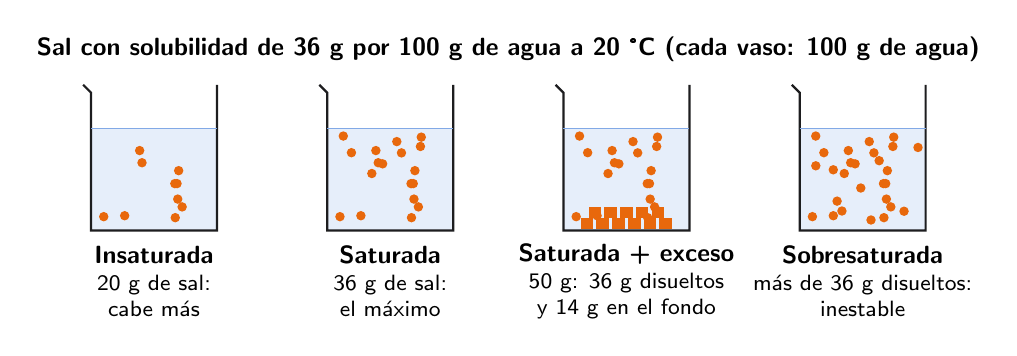
\begin{tikzpicture}[font=\small]
\node[font=\small\bfseries] at (4.5,2.3) {Sal con solubilidad de 36 g por 100 g de agua a 20 °C (cada vaso: 100 g de agua)};
\vaso{0}{10}
\node[align=center,font=\footnotesize] at (0,-0.65) {\textbf{\small Insaturada}\\20 g de sal:\\cabe más};
\vaso{3}{18}
\node[align=center,font=\footnotesize] at (3,-0.65) {\textbf{\small Saturada}\\36 g de sal:\\el máximo};
\vaso{6}{18}
\foreach \x in {-0.5,-0.3,...,0.5} \fill[nar] (6+\x-0.08,0.02) rectangle (6+\x+0.08,0.16);
\foreach \x in {-0.4,-0.2,...,0.4} \fill[nar] (6+\x-0.08,0.16) rectangle (6+\x+0.08,0.30);
\node[align=center,font=\footnotesize] at (6,-0.65) {\textbf{\small Saturada + exceso}\\50 g: 36 g disueltos\\y 14 g en el fondo};
\vaso{9}{27}
\node[align=center,font=\footnotesize] at (9,-0.65) {\textbf{\small Sobresaturada}\\más de 36 g disueltos:\\inestable};
\end{tikzpicture}
\end{document}
